\documentclass[12pt, a4paper, twocolumn]{article}

\usepackage[utf8]{inputenc}
\usepackage[T1]{fontenc}
\usepackage[polish]{babel}
\usepackage{csquotes}

% margines
\usepackage[left=1.6cm, right=1.6cm, top=2cm, bottom=2.5cm, columnsep=0.8cm]{geometry}

% czcionka
\usepackage{newtxtext, newtxmath}
\usepackage{microtype}

% grafiki
\usepackage{graphicx}
\usepackage{caption}
\usepackage{svg}
\usepackage{float}

% misc
\raggedbottom
\linespread{1.05}

% nagłówki
\usepackage{titlesec}
\titleformat{\section}{\fontsize{14}{16}\bfseries}{\thesection.}{0.5em}{}
\titleformat{\subsection}{\fontsize{12}{14}\bfseries}{\thesubsection.}{0.5em}{}
\titlespacing*{\section}   {0pt}{3ex plus 1ex minus .2ex}{1.5ex}
\titlespacing*{\subsection}{0pt}{2ex plus 1ex minus .2ex}{1.2ex}

% linki
\usepackage[colorlinks=true, linkcolor=blue, citecolor=blue, urlcolor=blue]{hyperref}

% bibliografia
\usepackage[
  backend=biber,
  style=numeric,
  sorting=none
]{biblatex}
\addbibresource{bibliografia.bib}

\begin{document}

\twocolumn[{%
  % nagłówek
  \noindent{\small Politechnika Warszawska - Wydział Elektryczny \hfill Projekt Indywidualny 2026}
  \vspace{0.6cm}

  \begin{center}
    % tytuł
    {\LARGE\bfseries Analiza metod geometrycznych wspomagania modelowania 3D\\[0.6cm]}

    {\large Kajetan Wójcik$^1$ \quad prof.\ dr.\ hab.\ inż.\ Dariusz Sawicki$^2$\\[0.4cm]}

    {\small
      $^1$Informatyka Stosowana, sem. 4, 333590\quad
      $^2$Prowadzący projekt, IETiSIP
    }
  \end{center}
  \vspace{0.7cm}

  % linia1
  \noindent\rule{\textwidth}{0.4pt}
  \vspace{0.3cm}

  % strzeszczenie
  \noindent\textbf{Streszczenie}\\[0.2cm]
  \noindent\textit{Praca przedstawia przegląd metod geometrycznych stosowanych w modelowaniu i wizualizacji trójwymiarowej. Omówiono trzy główne podejścia do reprezentacji geometrii: siatki wielokątów (mesh), powierzchnie parametryczne (NURBS) oraz funkcje odległości ze znakiem (SDF). Następnie przeanalizowano algorytmy proceduralnego generowania i modyfikowania geometrii, w tym szumy i powierzchnie subdywizyjne. Ostatnia część poświęcona jest metodom interakcji z powierzchnią, ze szczególnym uwzględnieniem algorytmu \textit{Marching Cubes} oraz analizy kolizji.}
  \vspace{0.3cm}

  \noindent\textbf{Słowa kluczowe:} modelowanie geometryczne, reprezentacja geometrii, generowanie proceduralne, grafika komputerowa 3D
  \vspace{0.3cm}

  % linia2
  \noindent\rule{\textwidth}{0.4pt}
  \vspace{0.8cm}
}]

\section{Wprowadzenie}
\label{sec:intro}

Grafika komputerowa 3D znajduje zastosowanie w niemal każdej dziedzinie, od przemysłu rozrywkowego, przez architekturę, aż do medycyny, gdzie pomaga wizualizować obiekty trójwymiarowe. Modelowanie geometryczne jest jednym z jej współczesnych fundamentów. Sposób w jaki komputer reprezentuje i przetwarza kształty trójwymiarowe ma bezpośredni wpływ na jakość obrazu, wydajność obliczeniową oraz możliwości edycji i animacji obiektów.

Celem pracy jest przegląd i analiza metod stosowanych do wspomagania modelowania geometrycznego. Omówiono trzy główne obszary, które zostały wybrane do analizy, ponieważ reprezentują komplementarne elementy modelowania geometrycznego: sposób przechowywania geometrii, metody jej generowania i modyfikacji oraz sposoby interakcji.

Rozdział 2 przedstawia sposoby reprezentacji geometrii. Rozdział 3 poświęcony jest proceduralnemu generowaniu geometrii. Rozdział 4 opisuje algorytmy stosowane na modelach.

Praca opiera się na przeglądzie literatury naukowej z zakresu grafiki komputerowej, obejmującej książki jak i artykuły konferencyjne publikowane na SIGGRAPH\footnote{Special Interest Group on Computer Graphics and Interactive Techniques - największa coroczna konferencja naukowa z zakresu grafiki komputerowej} oraz w czasopismach naukowych.

 \section{Klasyfikacje reprezentacji geometrii}
\label{sec:rep}
Wybór reprezentacji geometrycznej określa dopuszczalne operacje oraz strukturę danych przechowywanych w pamięci. Dzieli się na dwie główne kategorie: jawne (w tym parametryczne) oraz uwikłane \cite{botsch2010, piegl1997}.

Reprezentacje jawne i parametryczne definiują powierzchnię poprzez podanie współrzędnych punktów. Jawne stosują funkcję, która mapuje przestrzeń trójwymiarową na dwuwymiarową, a parametryczne opisują punkty powierzchni poprzez niezależne zmienne pomocnicze.

Modele uwikłane opisują powierzchnię jako zbiór punktów spełniających równanie $f(x,y,z) = 0$, gdzie funkcja zwraca wartość skalarną dla każdego punktu przestrzeni trójwymiarowej.

W niniejszej pracy omówiono trzy modele geometryczne. Siatki trójkątów i powierzchnie NURBS\footnote{Non-Uniform Rational Basis Splines} należą do reprezentacji parametrycznych. Natomiast funkcje odległości ze znakiem (SDF\footnote{Signed Distance Function}) przedstawiają podejście uwikłane.

Powodem wyboru siatek trójkątów, powierzchni NURBS oraz funkcji odległości ze znakiem jako obiekty mojej analizy, była chęć przedstawienia trzech fundamentalnych a jednocześnie różnych podejść reprezentacji geometrii. Każda z nich wspiera inny proces, czy to precyzyjne modelowanie inżynieryjnie czy modelowanie rzeźbiarskie. Zbadanie tych podejść pozwoli na analizę porównawczą metod reprezentacji geometrii trójwymiarowej.

Reprezentacje mają swoje zalety i wady, co wymusza wybór odpowiedniego rozwiązania dla danego problemu, czy wymagana jest precyzja krzywych, jakie operacje muszą być wspierane oraz jakie są ograniczenia obliczeniowe. Każde z tych zagadnień wpływa na decyzje o wyborze reprezentacji danych.

\subsection{Siatki trójkątów}
\label{sec:mesh}

\begin{figure}[h!]
    \centering
    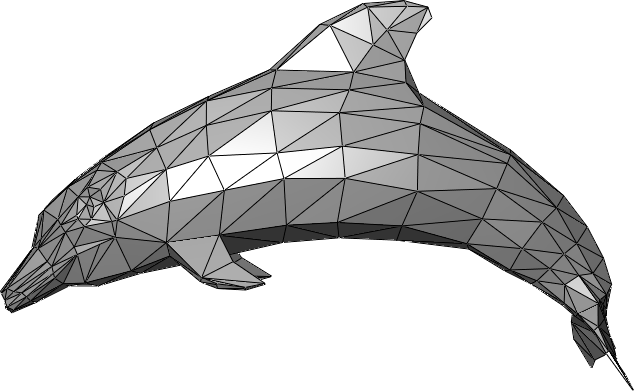
\includegraphics[width=\columnwidth]{media/Dolphin_triangle_mesh.png}
    \caption{Siatka modelu delfina. Chrschn, Public domain, via Wikimedia Commons}
    
\end{figure}

\paragraph{Definicja i historia}
Standard, który został przyjęty na kartach graficznych to siatki trójkątów. Trzy wierzchołki, które nie są współliniowe, wyznaczą dokładnie jedną płaszczyznę, co w wypadku czworokątów nie jest zawsze gwarantowane.

Siatka trójkątów jest zdefiniowana jako $M=(V,E,F)$, gdzie $V = \{v_1,...,v_{|V|}\}$ to zestaw wierzchołków, $E = \{e_1,...,e_{|E|}\}$ to krawędzie między wierzchołkami a $F = \{f_1,...,f_{|F|}\}$ to zestaw ścian. Każda ściana jest określona przez unikalną trójkę wierzchołków należących do zbioru $V$. W najprostszych strukturach krawędzie nie są przechowywane w pamięci, ale wynikają z definicji ścian.

Każdy z trójkątów w siatce posiada wektor normalny, który wyznacza się przez iloczyn wektorowy krawędzi:
\begin{equation}
    \mathbf{n} = (v_2 - v_1) \times (v_3 - v_1)
\end{equation}
Kierunek normalnej jest określony przez kolejność wierzchołków i pozwala określić orientację, co jest podstawą technik takich jak \textit{back-face culling}, który jest używany przez karty graficzne do odrzucania niewidocznych powierzchni w trakcie renderowania.

Dla zamkniętej siatki spełniającej warunek rozmaitości 2-wymiarowej zachodzi tożsamość Eulera:
\begin{equation}
    V - E + F = 2
\end{equation}
gdzie $V$ to liczby wierzchołków, $E$ krawędzi i $F$ ścian, spełnienie warunku jest wymagane przez większość algorytmów operujących na siatkach \cite{botsch2006}.

Przed przejściem do struktur danych warto wyjaśnić rozmaitość 2-wymiarową, jest to pojęcie z zakresu topologii, które pojawia się w literaturze dotyczącej reprezentacji geometrii trójwymiarowej. W kontekście siatek wielokątowych wymaga spełnienia dwóch warunków. Pierszy z nich to, że każda krawędź może należeć do maksymalnie dwóch trójkątów, a drugi mówi że otoczenie każdego wierzchołka musi tworzyć pojedyńczy wspólny wachlarz wielokątów. Krawędzie należące do dokładnie jednego trójkąta są definicją otworu, w przypadku siatek zamkniętych każda krawędź jest współdzielona przez dokładnie dwa trójkąty, co gwarantuje brak dziur \cite{bloom1997}.

\paragraph{Struktury danych}

Dobór struktury danych do przechowywania siatki wpływa na sprawność operacji lokalnych.

Najprostsza struktura to \textit{Indexed Face Set}, przechowująca listę wierzchołków oraz listę ścian jako trójki indeksów wierzchołków. Pozwala to na uniknięcie duplikowania współrzędnych wierzchołków współdzielonych przez sąsiednie trójkąty. Natomiast wadą jest brak możliwości efektywnego odpytania o sąsiedztwo. Aby wyznaczyć sąsiednie ściany danego wierzchołka wymogiem jest przeszukanie całej listy \cite{kettner1998}. 

W celach optymalizacji stosowane są rozszerzone struktury danych, które przetrzymują wskaźniki do sąsiednich elementów.

\textit{Winged-Edge Data Structure} przechowuje dla każdej krawędzi osiem referencji: wierzchołek początku i końca, lewą i prawą ścianę, oraz cztery sąsiednie krawędzie, tzw. "skrzydła" od których wynosi się nazwa struktury. Wadą takiego podejścia jest fakt, że krawędź nie posiada orientacji, przy przechodzeniu przez siatkę potrzebna jest weryfikacja kierunku ruchu \cite{kettner1998}.

\textit{Half-edge Data Structure} powstała jako rozwiązanie problemów obejmujących poprzednio omówioną strukturę. Polega na podzieleniu każdej krawędzi na dwie pół-krawędzie z przeciwnymi orientacjami, dzięki czemu zawsze znają własną stronę skierowania. Każda przechowuje wskaźniki do: wierzchołka do którego prowadzi, ściany po lewej stronie, następnej i przeciwnej pół-krawędzi, sprawia to że przechodzenie po siatce jest jednoznaczne. Podobnie jak Winged-Edge, struktura \textit{half-edge} modeluje orientowalne 2-rozmaitości, przy czym orientacja jest opisana bezpośrednio w pół-krawędziach \cite{kettner1998}.

Wybór struktury innej niż IFS ma wyraźny wpływ na wydajność narzędzi do edycji. Algorytmy jak wygładzanie czy podział powierzchni wymagają częstego odpytywania o sąsiedztwo wierzchołków i modyfikowania topologii. W strukturze IFS\footnote{Indexed Face Set} znalezienie sąsiednich ścian wymusza przeszukanie całej listy, co przy modelach mających miliony trójkątów daje złożoność $O(F)$. Struktura taka jak \textit{half-edge} redukuje tę operację do $O(1)$.

\paragraph{Zastosowania}
Siatki trójkątów są stosowane niemal wszędzie gdzie wymagana jest reprezentacja geometrii 3D, zarówno w zastosowaniach w czasie rzeczywistym jak i w renderowaniu offline.

W grach komputerowych każdy obiekt sceny reprezentowany jest przez siatkę, ponieważ karty graficzne posiadają dedykowany sprzęt do rasteryzacji trójkątów. W animacji filmowej, studia takie jak Pixar, czy DreamWorks wykorzystują siatki jako format modeli postaci i środowisk. Druk 3D wykorzystuje format STL, oparty o listę trójkątów spełniających warunek rozmaitości 2-wymiarowej.

\paragraph{Zalety i wady}
Główną zaletą siatek trójkątów jest uniwersalność oraz natywne wsparcie sprzętowe kart graficznych, co czyni je dominującą reprezentacją geometrii w grafice komputerowej. Prostota struktury umożliwia efektywną implementację szerokiego zakresu algorytmów. Wadą natomiast jest charakter aproksymacyjny reprezentacji, wierne odwzorowanie gładkich krzywych powierzchni wymaga bardzo gęstej siatki, która jest obliczeniowo droga, lub zastosowania powierzchni podziału, takich jak algorytm Catmull-Clark, który iteracyjnie wygładza siatkę przez dodawanie nowych wierzchołków \cite{halstead1993}.

\subsection{Powierzchnie NURBS}
\label{sec:nurbs}

\paragraph{Definicja i historia}
Przed komputerami inżynierowie opisywali krzywe za pomocą fizycznych splajnów, czyli elastycznych listw trzymanych obciążnikami. Matematycznym odpowiednikiem są wielomiany, jednak mają poważne ograniczenia: nie pozwalają na precyzyjny opis krzywych stożkowych, a ich współczynniki nie są intuicyjne z geometrycznego punktu widzenia \cite{rogers2001}.

Pierre Bézier zaproponował reprezentację, która jest oparta na punktach kontrolnych. Niestety jego metoda miała wadę, przy złożonych kształtach wymagała wielomianów wysokiego stopnia, które są niestabilne numerycznie \cite{rogers2001}.

Rozwiązaniem stały się krzywe B-splajnowe. Składają się z wielu połączonych fragmentów wielomianów niskiego stopnia, a zakres wpływu punktów kontrolnych jest ograniczony za pomocą tablicy węzłów. Chociaż B-splajny pozbyły się niestabilności numerycznej, wciąż opierały się na wielomianach, przez co nie pozwalały na dokładny opis krzywych stożkowych \cite{rogers2001, piegl1997}.

Krzywe NURBS rozwiązują ten problem poprzez wprowadzenie wag do punktów kontrolnych, odpowiada to matematycznemu dodaniu czwartej współrzędnej. Krzywa powstaje poprzez rzut z przestrzeni czterowymiarowej, umożliwia to dokładny opis krzywych stożkowych \cite{piegl1997}.

\begin{figure}[h!]
    \centering
    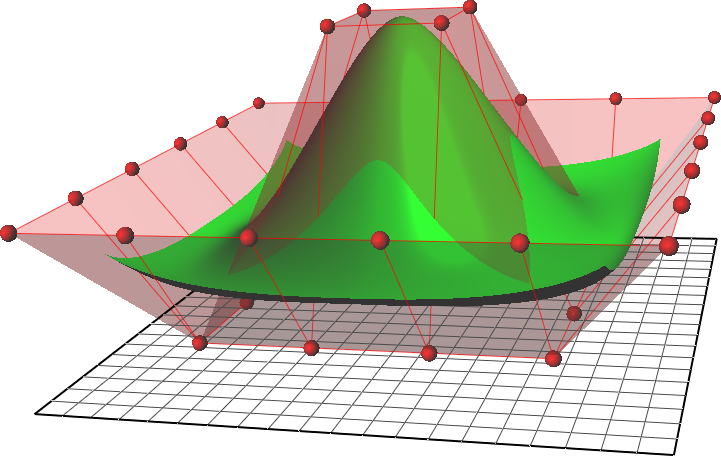
\includegraphics[width=\columnwidth]{media/NURBS_surface.png}
    \caption{Powierzchnia NURBS. Accountalive, CC BY-SA 3.0, via Wikimedia Commons}
    
\end{figure}

\paragraph{Zasada działania}
Krzywa NURBS o stopniu $d$ z punktami kontrolnymi $\mathbf{b}_0,\ldots, \mathbf{b}_n$, wagami $w_0,\ldots,w_n$ oraz tablicą węzłów $t_0,\ldots,t_m$ jest definiowana jako \cite{duncan2005}:
\begin{equation}
    \mathbf{B}(t) = \frac{\sum_{i=0}^{n} w_i \mathbf{b}_i N_{i,d}(t)}
    {\sum_{i=0}^{n} w_i N_{i,d}(t)}
\end{equation}
gdzie $N_{i,d}(t)$ to funkcje B-splajnu zdefiniowane na tablicy węzłów. Węzły $t_i$ są parametrami wyznaczającymi lokalizację funkcji, co oznacza, że każdy punkt kontrolny wpływa tylko na fragment odpowiadający jego przedziałowi, a nie na całą krzywą. 

Przekształcenia afiniczne stosuje się do krzywej NURBS poprzez zastosowanie ich na punkty kontrolne. Kształt krzywej można modyfikować przez zmianę pozycji punktów kontrolnych i przez zmianę ich wag, gdzie zwiększenie wagi przyciąga krzywą bliżej do danego punktu, jest to intuicyjnym rozwiązaniem. Krzywe NURBS są niezmienne zarówno przy przekształceniach afinicznych jak i rzucie perspektywicznym, co jest istotną właściwością dla zastosowań w grafice komputerowej \cite{piegl1997}.

\paragraph{Struktury danych}
Minimalna struktura danych, która opisuje krzywą NURBS zawiera: wielokąt kontrolny, który jest zestawem punktów kontrolnych wraz z wagami, stopień krzywej oraz tablice węzłów \cite{piegl1997}. Pełny zestaw danych obejmuje też najwyższe indeksy punktów kontrolnych i węzłów, jednak z perspektywy programisty działającego na gotowej krzywej wystarczy minimalna forma. W przypadku powierzchni NURBS struktura rozszerza się do siatki punktów kontrolnych $m \times n$, dwóch stopni oraz dwóch tablic węzłów.

\paragraph{Zastosowania}
Krzywe NURBS są stosowane głównie w miejscach gdzie jest wymagana precyzja opisu geometrii. Systemy CAD/CAM wykorzystują je jako podstawową reprezentację swoich krzywych i powierzchni, ponieważ dokładność jest tam konieczna, aby móc wytwarzać lub obrabiać części maszynowo. W przemysłach samochodowych i lotniczych NURBS umożliwia tworzenie powierzchni aerodynamicznych oraz przeprowadzanie akuratnych symulacji na modelach. Mimo dominacji siatek wielokątów w animacji i grach, każde profesjonalne oprogramowanie do modelowania trójwymiarowego obsługuje NURBS jako format.

\paragraph{Zalety i wady}
Główna zaleta krzywych NURBS to możliwość precyzyjnego opisu krzywych stożkowych takich jak okręgi czy elipsy, na co krzywe Béziera nie pozwalają. Modyfikacja kształtu dzięki węzłom, pozwala na edytowanie jedynie fragmentu krzywej bez przekształcania pozostałej części modelu. Następną zaletą jest fakt, że taka reprezentacja jest numerycznie stabilna w porównaniu do wielomianów wysokiego stopnia. 

Wadą natomiast jest nieintuicyjność punktów kontrolnych, ponieważ krzywa nie przechodzi przez te punkty, ale jest przez nie sterowana. Złożona topologia, jest trudna do ujęcia za pomocą krzywych NURBS. Pod względem implementacyjnym ta reprezentacja jest bardziej złożona niż siatki trójkątów \cite{piegl1997}.

Ważną przeszkodą powierzchni NURBS jest potrzeba na regularną siatkę punktów kontrolnych $m \times n$. Uniemożliwia ona swobodne modelowanie skomplikowanych obiektów, trudne modele potrzebują ręcznego łączenia wielu osobnych czworokątnych łat NURBS. Proces jest numerycznie niestabilny, co często prowadzi do powstawania dziur na złączach, jest to jedną z większych wad względem siatek wielokątnych.

\subsection{Funkcje odległości ze znakiem (SDF)}
\label{sec:sdf}

\paragraph{Definicja i historia}
Reprezentacja uwikłana opisuje powierzchnie jako zbiór punktów, które spełniają równanie $f(\mathbf{x}) = 0$. Zależnie od znaku zwróconej przez funkcję wartości jesteśmy w stanie określić względne położenie punktu od powierzchni. $f(\mathbf{x}) < 0$ oznacza wnętrze bryły, $f(\mathbf{x}) > 0$ oznacza że punkt jest na zewnątrz, natomiast $f(\mathbf{x}) = 0$ leży dokładnie na powierzchni \cite{osher2003}

Ta właściwość daje przewagę nad reprezentacjami jawnymi w sprawdzaniu przynależności punktu do obiektu. Modele jawne wymagają rzut promienia, który zlicza ilość przecięć z powierzchnią, parzysta liczba oznacza, że punkt jest na zewnątrz obiektu, a nieparzysta wewnątrz. W reprezentacji uwikłanej potrzeba jedynie obliczyć $f(\mathbf{x})$ i sprawdzić znak \cite{osher2003}.

\begin{figure}[h!]
    \centering
    \includesvg[width=\columnwidth]{media/SDF_duck.svg}
    \caption{Wizualizacja dyskretnego pola odległości ze znakiem w kształcie kaczki. Drummyfish, CC0, via Wikimedia Commons}
\end{figure}

\paragraph{Zasada działania}
Funkcja odległości ze znakiem jest przypadkiem reprezentacji uwikłanej, gdzie wartość funkcji zwraca odległość do najbliższej powierzchni i jest definiowana ogólnym wzorem:
\begin{equation}
    d(\mathbf{x}) = \min_{\mathbf{x'} \in \partial\Omega} 
    \|\mathbf{x} - \mathbf{x'}\|
\end{equation}
gdzie $\partial\Omega$ to powierzchnia obiektu. Gradient funkcji $\nabla d(\mathbf{x})$ jest wersorem, czyli wektorem jednostkowym i wskazuje kierunek najbliższego punktu na powierzchni \cite{osher2003}.

\begin{figure}[h!]
    \centering
    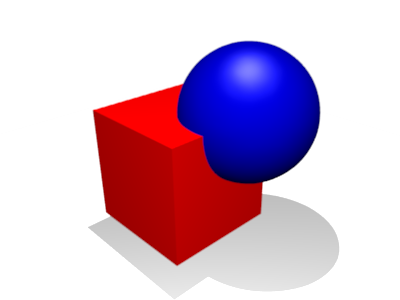
\includegraphics[width=0.32\columnwidth]{media/Boolean_union.png}\hfill
    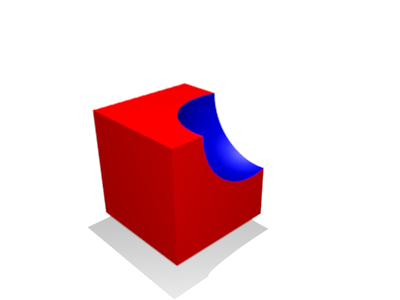
\includegraphics[width=0.32\columnwidth]{media/Boolean_difference.png}\hfill
    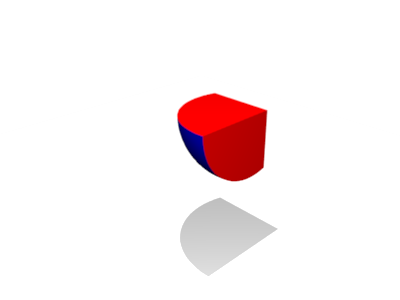
\includegraphics[width=0.32\columnwidth]{media/Boolean_intersect.png}
    
    \caption{Wyniki operacji boolowskich wykonanych na kostce i kuli: sumy, różnicy i części wspólnej}
\end{figure}


Reprezentacje uwikłane dają możliwość wykonywania operacji konstruktywnej geometrii brył CSG\footnote{Constructive Solid Geometry} przez proste operacje. Dla dwóch brył opisanych funkcjami $f_1$ i $f_2$ operacje Boola można zdefiniować jako:
\begin{align}
    f_1 \cup f_2 &= \min(f_1(\mathbf{x}),\ f_2(\mathbf{x})) \\
    f_1 \cap f_2 &= \max(f_1(\mathbf{x}),\ f_2(\mathbf{x})) \\
    f_1 \setminus f_2 &= \max(f_1(\mathbf{x}),\ -f_2(\mathbf{x}))
\end{align}

\paragraph{Struktury danych}
Najprostszą do zaimplementowania strukturą danych wykorzystywaną do przechowywania SDF jest gęsta siatka wokseli, gdzie woksel to najmniejszy element przestrzeni. Przestrzeń wokół obiektu jest dzielona na regularną trójwymiarową siatkę sześcianów, gdzie każdy woksel przechowuje jedną wartość zmiennoprzecinkową: odległość od najbliższej powierzchni. Taka struktura posiada dostęp do danych w czasie stałym $O(1)$ jako że jest stworzona z tablic, natomiast przynosi to też złożoność pamięciową rzędu $O(N^3)$, co wyklucza ją z użytkowania przy wysokich rozdzielczościach.

Zauważono właściwość, że wartości SDF bliskie zeru pojawiają się tylko w pobliży powierzchni, co doprowadziło do utworzenia metody wąskiego pasma \cite{sethian1999}. Technika polega na przechowywaniu precyzyjnych danych tylko w obszarze blisko powierzchni $f(\mathbf{x}) = 0$ i pomijaniu dalszych stref. Strukturą danych która odwzorowuje ten pomysł jest drzewo ósemkowe. Gdy dany obszar jest daleki od obiektu, to pozostaje niepodzielony jako liść drzewa. Przestrzeń która przecina powierzchnie jest rekurencyjnie dzielona na osiem sześcianów, do momentu osiągnięcia żądanej rozdzielczości. W reprezentacji drzewa korzeniem jest cała przestrzeń, a liście to obszary nie wymagające podziału.

\begin{figure}[h!]
    \centering
    \includesvg[width=\columnwidth]{media/Octree2.svg}
    \caption{Struktura drzewa ósemkowego. WhiteTimberwolf, CC BY-SA 3.0, via Wikimedia Commons}
\end{figure}

\paragraph{Zastosowania}
Funkcje odległości ze znakiem mają szerokie zastosowanie w grafice komputerowe i symulacjach fizycznych. Technika \textit{ray marching} używa SDF do adaptacji długości kroku wzdłuż promienia bez ryzykowania ominięcia powierzchni co przyśpiesza obliczenia w porównaniu do klasycznego \textit{ray castingu} \cite{hart1996}. SDF umożliwia też wydajne obliczanie miękkich cieni i okluzji, ponieważ odległość od powierzchni jest wbudowana w metodę. W symulacjach SDF jest wykorzystywany do detekcji i obsługi kolizji, szczególnie w symulacjach cieczy lub tkanin. Metoda cieszy się popularnością w robotyce.

\paragraph{Zalety i wady}
Główną zaletą SDF jest zwięzłość reprezentacji, powierzchnia jest w tej metodzie zdefiniowana analitycznie lub jako gęste pole wartości. Kolejną istotną zaletą jest możliwość wykorzystywania operacji takich jak CSG, czy trywialne obliczanie normalnych za pomocą gradientu. Jest to główna metoda wykorzystywana do algorytmów detekcji i kolizji, dzięki dostępowi do informacji w czasie stałym.

Wadą SDF są jej struktury danych, gdzie dla siatki wokseli złożoność pamięciowa wynosi $O(N^3)$. Struktury adaptacyjne takie jak drzewa ósemkowe ograniczają ten problem, ale kosztem złożoności czasowej i lokalności danych dla pamięci podręcznej procesora.

Ważnym ograniczeniem jest koszt jaki potrzeba podjąć przy aktualizacji danych. Dla obiektów dynamicznych konieczne jest przeliczenie pola odległości, co dla algorytmu \textit{Fast Sweeping Method} wynosi $O(N^3)$, a dla algorytmu \textit{Fast Marching Method} $O(N^3 \log N)$ \cite{sethian1999}. Sprawia to że SDF są trudne do stosowania w sytuacjach, gdy występuje częsta zmiana geometrii.

\subsection{Wnioski}
\label{sec:wnioski}

Każda z opisanych metod reprezentacji geometrii trójwymiarowej, siatki wielokątów, krzywe NURBS i reprezentacje oparte na funkcjach odległości ze znakiem posiadają swoje wady i zalety, które są wynikiem ich podstaw matematycznych. 

Wybór jednej z metod nad drugą nie powinien być kwestią preferencji, ale wynikać z analizy ograniczeń podanego problemu. Limity mogą być o charakterze obliczeniowym, takim jak budżet pamięci i czas albo geometrycznym, gdzie kształt musi mieć dokładną reprezentację charakterystycznej powierzchni, albo nawet narzucony format przez wymagane narzędzia. W praktyce to właśnie ograniczenia, a nie zalety mają rolę filtra, szybciej wyeliminują metody niż zalety wskażą optymalną metodę. Dopiero po zawężeniu listy możliwych rozwiązań, można zacząć porównywać różnice w wydajności i charakterze metod.

Pierwszym kryterium porównania jest swoboda topologiczna, czyli w jakim stopniu struktura reprezentacji ogranicza możliwości opisu obiektu. Siatki nie narzucają żadnych ograniczeń i pozwalają na złożone topologie. NURBS natomiast jest ograniczony ze względu na swoją definicję matematyczną, przez co skomplikowane topologię wymagają wykorzystania wielu łatek, między którymi pojawia się potrzeba zarządzania złączami, aby móc utworzyć reprezentację modelu. Funkcje odległości ze znakiem z kolei najlepiej z opisanych metod obsługują dynamiczne zmiany topologii, dzięki możliwości wykorzystywania operacji boolowskich i scalaniu powierzchni. Ograniczenie tej reprezentacji natomiast pojawia się podczas ekstrakcji danej geometrii, algorytmy wykorzystywane na tej metodzie mogą wprowadzać artefakty.

Precyzja w kontekście reprezentacji geometrii oznacza dokładność odwzorowania matematycznego modelu, względem otrzymanego kształtu obiektu, oraz ciągłość powierzchni opisaną klasami C0, C1 i C2. Siatki wielokątów gwarantują ciągłość C0, czyli przejście tylko między krawędzią styczności dwóch powierzchni, gdzie wciąż występuje ostre załamanie. Normalne są nieciągłe na krawędziach, natomiast dokładność wzrasta wraz z zagęszczeniem siatki. Reprezentacja NURBS jest dokładna ze względu na nature swojego opisu matematycznego, krzywe i powierzchnie są wyrażone analitycznie, co sprawia że ciągłość C2 - druga pochodna jest ciągła na złączeniu. Dzięki tym zależnością krzywe NURBS dominują w projektowaniu przemysłowym. SDF są analitycznie dokładne, natomiast po dyskretyzacji precyzja jest ograniczona poprzez rozdzielczość siatki wokseli. Gradient umożliwia dokładne kalkulację wektorów normalnych, ale tylko w miejscach gdzie pole odległości jest właściwie zdefiniowane. Spośród trzech omówionych metod NURBS jest jedyną która nie opiera się na przybliżeniach.



\section{Proceduralne generowanie geometrii}
\label{sec:gen}
Reprezentacje opisane w rozdziale \ref{sec:rep} definiują jak geometria jest przechowywana i przetwarzana. Proceduralne generowanie dostarcza algorytmy, które tworzą lub zmieniają kształty według danych zasad. Pozwalają one na modyfikację bez ręcznego modelowania każdego szczegółu. Ten rozdział omawia dwa różne podejścia: powierzchnie subdywizyjne, które wygładzają istniejącą siatkę, oraz szumy, które generują dane od podstaw.

\subsection{Powierzchnie Subdywizyjne}
\label{sec:sub}
Powierzchnie subdywizyjne stanowią most między prostotą siatek o małej ilości wielokątów a gładkością powierzchni opartych na krzywych NURBS. Zamiast przetrzymywać duże ilości danych gęstej siatki, metoda przechowuję grubą siatkę bazową, która opisuje intencję kształtu a szczegóły produkuje proceduralnie.

\paragraph{Definicja i historia}
Siatki składające się z małej ilości wielokątów, nie pozwalają na skrupulatne odwzorowanie gładkich powierzchni. Chociażby krawędzie między ścianami są zawsze widoczne niezależnie od metody cieniowania. Powierzchnie subdywizyjne starają się rozwiązać ten problem poprzez zagęszczanie pierwotnej siatki iteracyjnie według zdefiniowanych zasad.

Edwin Catmull wynalazł metodę na generowanie powierzchni sześciennych dla dowolnych topologii. Natomiast nie był w stanie udowodnić, że powierzchnia jest stabilna w każdym punkcie, zdecydował się więc nie implementować jej. Jim clark wdrożył jego metodę i udowodnił empirycznie, że powierzchnia jest stabilna. W ten sposób pierwszym schematem, który powstał dla powierzchni czworokątnych był algorytm Catmull-Clark. Został on przedstawiony w 1978 roku jako uogólnienie rekursywnego podziału bikubicznych powierzchni B-splajnowych dla siatek o dowolnej topologii \cite{catmull1978}. Metoda jest zaprojektowana do produkowania powierzchni o ciągłości C2 wszędzie oprócz punktów nadzwyczajnych, w których spada do C1.

Schemat Loopa, został zaproponowany przez Charlesa Loopa w jego pracy magisterskiej z 1987 roku. Rozwiązuje on w niej ten sam problem co Catmull-Clark, lecz dla siatek trójkątnych \cite{warren2001, zorin2000}. Podobnie jak Catmull-Clark opiera się na uogólnieniu funckji B-splajnowych i produkuje powierzchnie z ciągłością C2 wszędzie poza punktami nadzwyczajnymi, gdzie wynosi C1.

Wierzchołek nadzwyczajny jest takim, który ma walencję, czyli liczbę przylegających krawędzi do wierzchołka, inną niż cztery. W standardowych sekcjach siatki, powierzchnia graniczna jest powierzchnią B-splajnową \cite{catmull1978, hughes2013}.

\paragraph{Zasada działania}
Algorytm Catmull-Clark działa na siatce czworokątów i iteracyjnie wprowadza trzy rodzaje nowych wierzchołków. Punkt ściany $\mathbf{f}$ to średnia wszystkich wierzchołków, które definiują daną ścianę. Punkt krawędzi $\mathbf{e}$ jest średnią dwóch krańców danej krawędzi oraz dwóch punktów ścian, które sąsiadują z daną krawędzią. Nową pozycję istniejącego wierzchołka $\mathbf{v}$ wyznacza się przez:
\begin{equation}
    \mathbf{v}' = \frac{\mathbf{Q}}{n} + \frac{2\mathbf{R}}{n} 
    + \frac{(n-3)\mathbf{S}}{n}
\end{equation}
gdzie $n$ to walencja, $\mathbf{Q}$ to średnia nowych punktów ścian które przylegają do wierzchołka, $\mathbf{R}$ to średnia punktów środkowych przylegających krawędzi, i $\mathbf{S}$ jest starą pozycją wierzchołka \cite{catmull1978}.

Po obliczeniu wierzchołków, siatka jest modyfikowana przez połączenie punktów ścian z punktami krawędzi oraz punktów krawędzi z nowymi wierzchołkami. Każdy czworokąt jest podzielony na cztery mniejsze, co sprawia że każda iteracja zwiększa ilość ścian czterokrotnie.

\begin{figure}[h!]
    \centering
    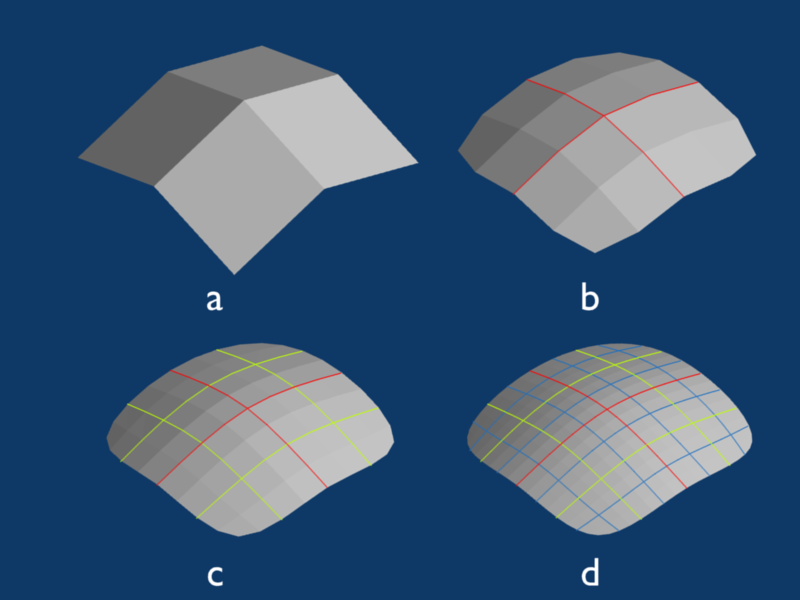
\includegraphics[width=0.8\columnwidth]{media/Catmull-Clark.png}
    \caption{Wizualizacja podziału algorytmem Catmull-Clark. Banlu Kemiyatorn, via Wikimedia Commons}
    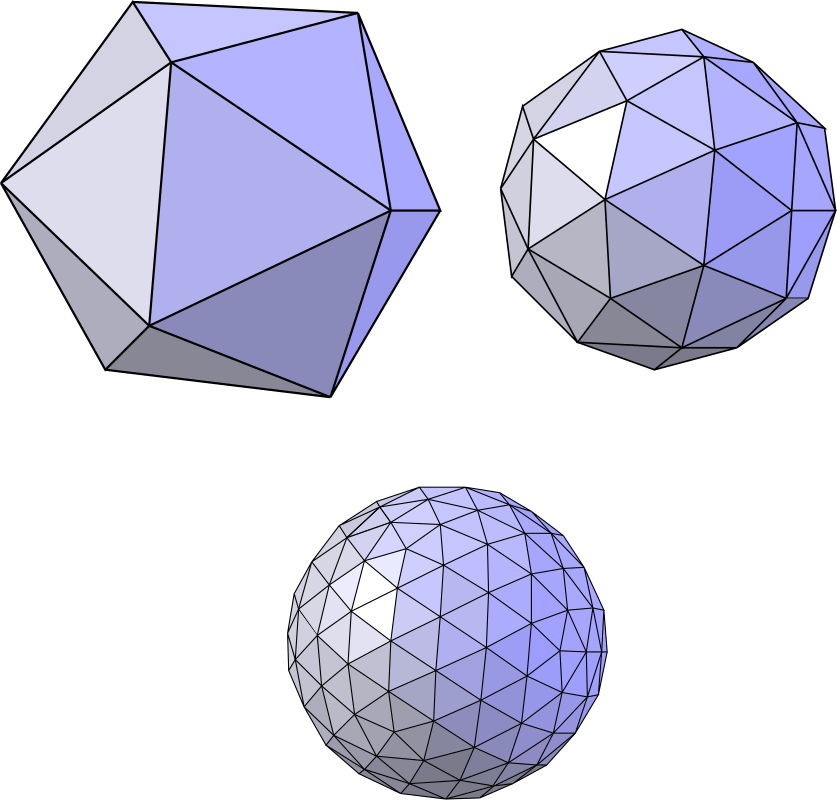
\includegraphics[width=0.8\columnwidth]{media/Loop.png}
    \caption{Wizualizacja podziału algorytmem Loopa. Simon Fuhrmann, CC BY-SA 3.0, via Wikimedia Commons}
    \label{fig:catmull}
\end{figure}

\paragraph{Warianty}
Schematy można podzielić na aproksymujące i interpolacyjne, kategoryzacja zależy od tego czy wierzchołki siatki bazowej są zachowane w powierzchni granicznej. W modelach aproksymujących, takich jak Catmull-Clark i Loop, wierzchołki są przesuwane w każdej iteracji, a punkty kontrolne nie leżą na powierzchni granicznej, natomiast są one jej przybliżeniem. W schematach interpolacyjnych, takich jak Modified Butterfly i Kobbelt \cite{warren2001}, wierzchołki siatki bazowej nie są modyfikowane i powierzchnia graniczna dokładnie przechodzi przez punkty kontrolne.

Interpolacja pozwala na bezpośrednią kontrolę punktów, które leżą na końcowej powierzchni, co upraszcza obliczenia. Niestety natomiast jakość powierzchni interpolacyjnych jest niższa niż aproksymujących, zbiegają wolniej do granicy i są bardziej podatne na artefakty \cite{zorin2000}.


\paragraph{Zastosowania}
Powierzchnie podziału są rozlegle wykorzystywane w animacji filmowej. Pixar wprowadził je do produkcji przy \textit{Geri's Game} (1997), a dwa lata później wydali artykuł w którym opisali szczegóły \cite{derose1998}. Główną motywacją był problem z deformacją, animowane postacie wymagają gładkich powierzchni przy zginaniu stawów. W tym wypadku gęste siatki wprowadzają artefakty na krawędziach. Podział siatki z niską ilością wielokątów rozwiązuje ten problem.

Programy do modelowania trójwymiarowego takie jak Blender czy Maya, wykorzystują algorytm Catmull-Clark jako standardowy modyfikator do użytku. Artysta może modelować siatkę o niskiej rozdzielczości a podział jest zastosowany przy renderowaniu. W grach komputerowych zastosowanie jest rzadsze przez koszt obliczeniowy w czasie rzeczywistym.

\paragraph{Zalety i wady}
Jedną z głównych zalet powierzchni subdywizyjnych jest kompaktowość reprezentacji, złożone topologie mogą być opisane siatkami z małą ilością wierzchołków. Inną zaletą jest gładkość powierzchni granicznej, która jest zagwarantowana matematycznie oraz fakt, że edycja siatki jest intuicyjna, ponieważ artysta może kontrolować bezpośrednio punkty kontrolne.

Ograniczeniem tej metody jest trudność w kontrolowaniu ostrych krawędzi, ponieważ algorytm polega na wygładzaniu geometrii co wymusza wykorzystywanie dodatkowych technik. Kolejną wadą jest koszt obliczeniowy, który wraz z liczbą iteracji rośnie wykładniczo. Dodatkowo punkty nadzwyczajne wprowadzają artefakty przez zaburzenie ciągłości w ich otoczeniu \cite{catmull1978}.

\subsection{Szumy Proceduralne}
Szum Perlina i inne szumy proceduralne rozwiązują inny problem niż powierzchnie subdywizyjne, zamiast modyfikować geometrię która już istnieje, generują dane bez ręcznego modelowania. Są one fundamentalną techniką w każdym miejscu gdzie jest potrzeba na kontrolowaną losowość.

\paragraph{Definicja i historia}
Ken Perlin opracował funkcję szumu pracując nad efektami wizualnymi do filmu \textit{TRON} (1982) w \textit{Information International Inc}. Celem było stworzenie tekstur proceduralnych, które wyglądają organicznie. Dotychczasowe metody opierały się na białym sumie, który nie ma żadnej koherencji przestrzennej i jest całkowicie losowy. W papierze \cite{perlin1985} z 1985 Perlin opisuje system teksturowania, którego szum jest częścią. Za swój algorytm Perlin dostał w 1997 nagrodę w Akademii Filmowej, co ukazuje jak dramatyczną zmianą było przedstawienie tej metody. W 2002 Perlin opublikował nowy artykuł \cite{perlin2002} w którym opisał poprawy, które wprowadził do swojego oryginalnego algorytmu, eliminując dwa ograniczenia z poprzedniej metody.

Steven Worley w 1996 roku zaproponował inne podejście do szumu proceduralnego \cite{worley1996}. Zamiast interpolować gradient na siatce, wartość funkcji zależy od odległości do najbliższego z losowo położonych punktów. Produkuje to wzory, które w kształcie przypominają organiczne struktury takie jak kamień lub skóra. W przeciwieństwie do szumu Perlina, który charakteryzuje się gładkimi przejściami.

\paragraph{Zasada działania}
Szum Perlina jest definiowany dla punktu $\mathbf{x} = (x, y, z)$ trzema krokami. Pierwszy to przypisanie pseudo-losowego wektora gradientu do każdego wierzchołka w siatce liczb całkowitych, które otaczają dany punkt. Gradienty są wyznaczone na podstawie wcześniej obliczonych tablicy permutacji $P$ i gradientów $G$. Tablica $P$ haszuje wierzchołki siatki do indeksu tablicy $G$, co pomimo pozornej losowości jest deterministyczne.

Kolejnym krokiem jest wyznaczenie iloczynu skalarnego między wektorem gradientu wierzchołka a wektorem odległości od tego wierzchołka do punktu $\mathbf{x}$. Następnie interpoluje się trójliniowo osiem takich wartości za pomocą funkcji:
\begin{equation}
    s(t) = 3t^2 - 2t^3
\end{equation}
Oryginalny algorytm posiada dwie wady. Pierwszą z nich jest niezerowa druga pochodna funkcji $s(t)$ dla $t=0$ i $t=1$, co wytwarza artefakty przy cieniowaniu. Drugą jest faworyzacja niektórych kierunków nad innymi spowodowana doborem gradientów \cite{perlin2002}.

Szum Worleya działa na innej zasadzie, wykorzystuje losowe rozrzucenie punktów $\mathbf{c}_i$, gdzie wartość funkcji jest wyznaczana przez odległość do najbliższego punktu:
\begin{equation}
    w(\mathbf{x}) = \min \|\mathbf{x} - \mathbf{c}_i\|
\end{equation}
Dzięki kombinacją odległości od pierwszego, drugiego oraz trzeciego najbliższego punktu, można otrzymać różne wizualnie szumy \cite{worley1996}.

\begin{figure}[h!]
    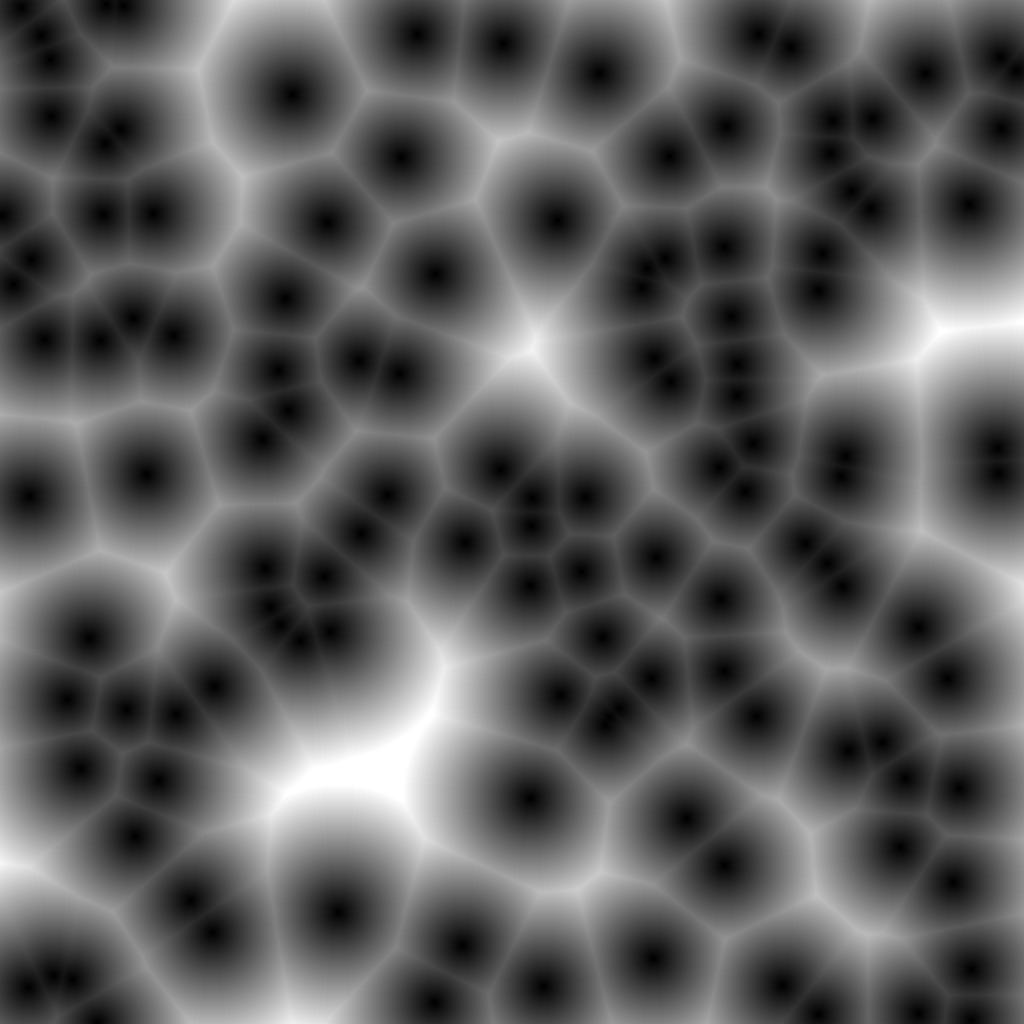
\includegraphics[width=\columnwidth]{media/Worley.jpg}
    \caption{Wizualizacja szumu Worleya. Rocchini, CC BY-SA 3.0, via Wikimedia Commons}
    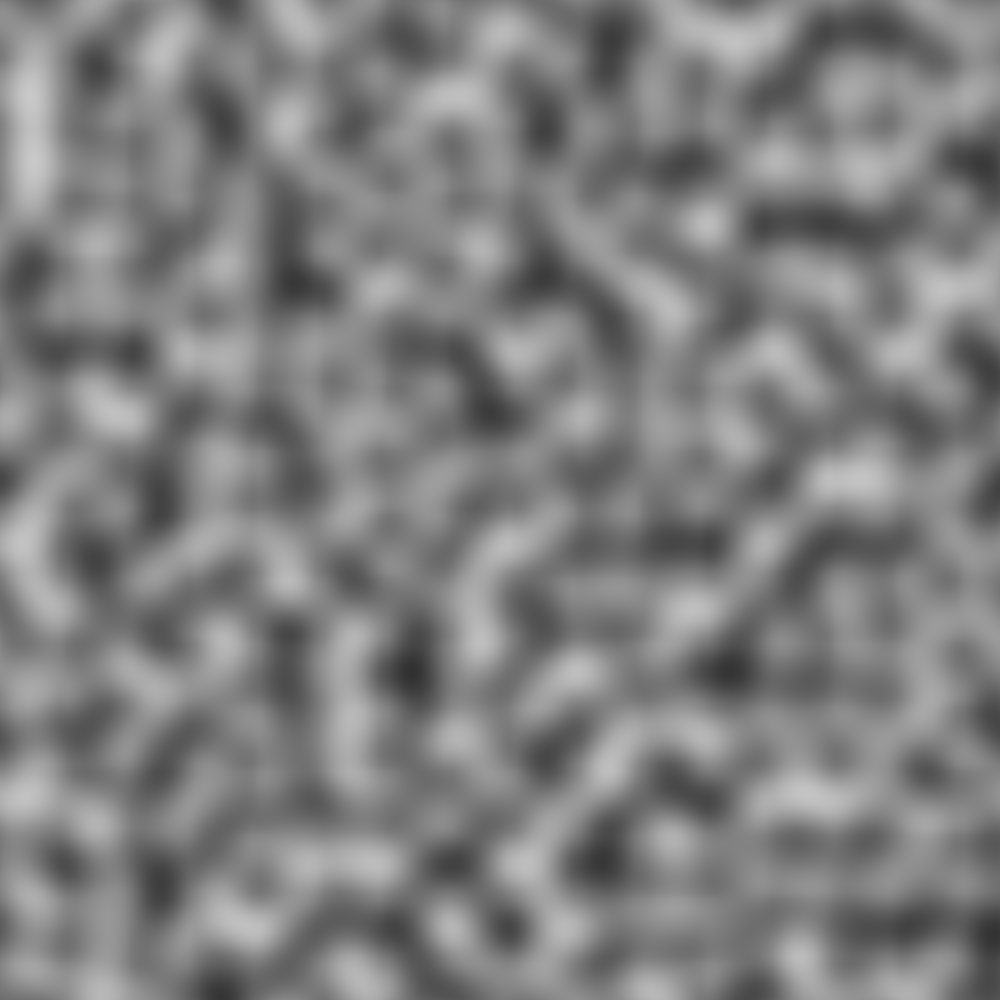
\includegraphics[width=\columnwidth]{media/Perlin.png}
    \caption{Wizualizacja szumu Perlina. Lord Belbury, CC0, via Wikimedia Commons}
\end{figure}

\paragraph{Warianty i rozszerzenia}
W swojej pracy z 2002 roku, Perlin opisał poprawiony algorytm szumu. Jedną z dwóch zmian którą wprowadził względem oryginału było zamienienie funkcji wygładzającej na:
\begin{equation}
    s(t) = 6t^5 - 15t^4 + 10t^3
\end{equation}
zapewnia ona ciągłość C2, czyli pierwsza i druga pochodna jest zerowa dla $t=0$ i $t=1$, dzięki czemu wyeliminowano artefakty cieniowania. Kolejną zmianą której dokonał Perlin było zastąpienie możliwych gradientów z pełni losowych na ograniczony zbiór, dzięki czemu pozbył się faworyzowania kierunków. Pomimo tych zmian algorytm wciąż jest około 10\% szybszy \cite{perlin2002}.

\textit{Simplex noise}, zaproponowany przez Perlina w \cite{perlin2001}, zastępuje siatkę sześcienną, siatką simpleksową. W trzech wymiarach simpleks jest czworościanem. Koszt obliczeniowy siatki sześciennej w $n$ wymiarach wymaga $2^n$ wierzchołków. W przeciwieństwie do tego siatka simpleksowa redukuje tą złożoność do $n+1$ wierzchołków, co dla trzech wymiarów zmniejsza osiem do czterech wymaganych wierzchołków.

\paragraph{Zastosowania}
Najbardziej znanym zastosowaniem szumu Perlina jest proceduralne generowanie terenu. Wartości szumu są próbkowane i tworzą mapę wysokości, która jest później przekształcana w siatkę trójkątną.

Innym kluczowym zastosowaniem są tekstury proceduralne. Wykorzystanie szumu Perlina pozwala na generowanie tekstur które imitują drewno, chmury czy ogień, więc wzory które wynikają naturalnie z przekształcenia szumu, a ciężko odwzorować ręcznie. Z kolei szum Worleya wykorzystuje się do teksturowania chociażby kamienia lub skóry.


\paragraph{Zalety i wady}
Główną zaletą szumów proceduralnych jest determinizm, gdzie ta sama wartość ziarna zawsze zwróci identyczny wynik, dzięki czemu można wykorzystywać generowane dane bez potrzeby przechowywania ich. W przeciwieństwie do szumu białego, szum Perlina posiada ciągłość przestrzenną co jest jego fundamentem. Drugą ważną zaletą jest niski i stały koszt obliczeniowy dla pojedynczego punktu.

Natomiast głównym ograniczeniem tych metod jest widoczna regularność przy niskich częstotliwościach, co ujawnia się jako powtarzająca struktura. Szum Perlina nie nadaje się do reprezentacji ostrych krawędzi, jako że wytwarza tylko gładkie i organicznie wyglądające przejścia. Mniejszą, ale znaczącą wadą jest kontrola, parametry pozwalają na ustalenie ogólnego charakteru wygenerowanych danych, ale nie pozwalają na sterowanie szczegółami.

\section{Interakcja z modelem}
\label{sec:int}
Reprezentacje geometryczne opisane w rozdziale \ref{sec:rep} oraz metody generowania omówione w rozdziale \ref{sec:gen} wymagają algorytmów które operują na na wygenerowanych przez nich danych. Ten rozdział opisuje praktyczne zastosowania takich algorytmów.

\subsection{Marching Cubes}
\label{sec:mar}
Algorytm przekształca dane między reprezentacjami uwikłanymi a siatką wielokątów, a dokładnie pole skalarne, takie jak SDF w siatkę trójkątów.

\paragraph{Definicja i historia}
\textit{Marching Cubes} jest algorytmem zaproponowanym przez Williama Lorensena i Harveya Cline'a w 1987 roku. Pierwotnie opublikowany w kontekście wizualizacji trójwymiarowych danych medycznych \cite{lorensen1987}.

W diagnostyce obrazy są złożone z wielu dwuwymiarowych przekrojów, które razem tworzą trójwymiarowy obiekt. Radiolodzy posiadają odpowiednie umiejętności do interpretacji przedstawionych w ten sposób danych, natomiast częstym wymogiem jest komunikacja z lekarzami, którzy nie mają w tym szkolenia. Ten problem utworzył zapotrzebowanie na czytelne modele trójwymiarowe wygenerowane z przekrojów. 

Przetwarzanie danych medycznych składało się z czterech kroków: pozyskanie przekrojów, filtrowanie obrazu, konstrukcji powierzchni i wyświetlenie jej, ten algorytm adresuje trzeci krok.

\paragraph{Zasada działania}
Metoda polega na przetwarzaniu pola skalarnego przez podział na regularne sześciany, czyli kostki i dla każdej z nich wyznacza jak izopowierzchnia przecina krawędzie. Izopowierzchnia jest definiowana jako trójwymiarowa powierzchnia wyznaczona za pomocą wszystkich punktów, które mają dokładnie tę samą wartość. 

Na każdy z ośmiu wierzchołków sześcianu zostaje nałożona wartość binarna: jeden jeśli wartość pola w tym punkcie $\ge$ wartości progowej, inaczej otrzymuje wartość zero. Przecięcie krawędzi przez powierzchnię występuje gdy jeden wierzchołek ma wartość jeden a drugi zero.

Jako że każda kostka ma osiem wierzchołków z dwoma możliwymi stanami, istnieje $2^8 = 256$ możliwych sposobów przecięcia. Algorytm enumeruje wszystkie przypadki i przetrzymuje je w tablicy przeglądowej. Natomiast dzięki podwójnej symetrii kostki możemy zredukować 256 przypadków do 15 wzorców \cite{lorensen1987}.

\begin{figure}[h!]
    \centering
    \includesvg[width=0.8\columnwidth]{media/MarchingCubes.svg}
    \caption{15 wzorców Marching Cubes. Jmtrivial, GPL, via Wikimedia Commons}
    
\end{figure}

W ostatnim kroku algorytm oblicza wektory normalne dla każdego z wierzchołków. Gradient pola $\nabla f$ jest prostopadły do izopowierzchni i jest wersorem normalnym dla SDF, co opisano w sekcji \ref{sec:sdf}.

\paragraph{Warianty}
Pierwsza optymalizacja zaproponowana w \cite{lorensen1987} wykorzystuje fakt, że sąsiednie kostki współdzielą swoje krawędzie. Przy liniowym przetwarzaniu przestrzeni wymagane jest tylko interpolowanie trzech nowych krawędzi na kostkę, pozostałe można odczytać z poprzednio obliczonych kostek. W tej metodzie występują specjalne warunki, gdzie kości znajdujące się na brzegach danych, nie mają poprzednio obliczonych wartości do wykorzystania. W praktyce przechowuje się tylko poprzedni piksel i przecięcia linii, aby zaoszczędzić na pamięci. Ten wariant przyśpiesza algorytm aż trzykrotnie.

Kolejnym usprawnieniem algorytmu jest zaimplementowanie operacji boolowskich. Pozwala to na wycinanie i zamykanie modeli, jak i również ekstrakcję różnych powierzchni \cite{lorensen1987}.

Algorytm \textit{Transvoxel} \cite{lengyel2010}, który został zaproponowany przez Lengyela, rozszerza \textit{Marching Cubes} o obsługę poziomów szczegółów LOD\footnote{Level Of Detail}. Rozwiązuje też problem artefaktowania na złączach między kośćmi z różnymi rozdzielczościami, co wykorzystywane jest przy generowaniu terenu z szumów.

\paragraph{Zastosowania}
Pierwsze zastosowanie w medycynie wciąż pozostaje aktualne. Rekonstrukcja trójwymiarowych modeli z danych wygenerowanych podczas tomografii komputerowej i rezonansu magnetycznego nadal opiera się na tej metodzie. W grafice komputerowej \textit{Marching Cubes} jest podstawową metodą stosowaną do ekstrakcji siatki z SDF. W kontekście generowania proceduralnego, ten algorytm jest mostem między szumem Perlina a finalną siatką.

\paragraph{Zalety i wady}
Główną zaletą algorytmu jest prosta implementacja i generalność, ponieważ działa on na dowolnym polu skalarnym, niezależnie od metody otrzymania go, czy to przez SDF, szum proceduralny lub dane diagnostyczne. Dzięki tablicy przeglądowej 256 różnych przypadków sprawia, że kostki przetwarzane są w czasie stałym $O(1)$.

Najważniejszym ograniczeniem tej metody jest niejednoznaczność występująca we wzorcach bazowych, dla niektórych z nich istnieje więcej niż jedno poprawne rozwiązanie. Kolejną wadą jest stała rozdzielczość siatki, algorytm nie adaptuje się do złożoności geometrii i przetwarza płaskie obszary z taką samą dokładnością co obszary złożone.

\subsection{Analiza kolizji na bazie SDF}
\label{sec:kol}
Detekcja kolizji rozwiązuje trzy powiązane ze sobą problemy: czy obiekty się przecinają, kiedy w trakcie ruchu wystąpiła kolizja, oraz gdzie i w jaki sposób obiekty się zetknęły \cite{ericson2004}. Reprezentacja SDF, opisana w \ref{sec:sdf} jest eleganckim rozwiązaniem pierwszego i trzeciego problemu poprzez wykorzystanie własności pól odległości.

\paragraph{Definicja i historia}
Na implementację detekcji kolizji wpływa wiele czynników. Reprezentacja geometryczna obiektów występujących w scenie determinuje możliwe do użycia algorytmy, rodzaj zapytań wpływa na koszt obliczeniowy, a właściwości symulacji takie jak liczba obiektów narzucają dodatkowe ograniczenia \cite{ericson2004}. Ważnym aspektem jest też wymóg działania w czasie rzeczywistym: w grze komputerowej drobna niedokładność będzie niezauważalna, natomiast podczas symulacji naukowej mały błąd może skompromitować całe badanie.

Zastosowanie SDF do detekcji kolizji jest wynikiem ich własności matematycznych. Pole odległości ze znakiem zawiera dokładnie tą informację którą wymaga detekcja, czyli odległość od powierzchni, przynależność punktu i kierunek normalnej \cite{bridson2008}.

\paragraph{Zasada działania}
Dla obiektu opisanego przez funkcję odległości $\phi$, wartość funkcji dla punktu $\mathbf{x}$, zwraca odległość do najbliższej powierzchni ze znakiem dodatnim na zewnątrz i ujemnym wewnątrz. Aby dla punktu $\mathbf{x}$ zapytać o wystąpienie kolizji, wystarczy obliczyć $\phi(\mathbf{x})$ i sprawdzić znak wartości. 

W praktyce wartości SDF są przetrzymywane na dyskretnej siatce wokseli, a zapytania o odległość punktu nie występującego na siatce są obsługiwane przez interpolację trójliniową. Otrzymany w ten sposób wynik jest przybliżeniem, ale wystarcza dla zastosowań symulacji fizycznych.

Zapytania o kolizję są operacjami o złożoności $O(1)$ po dyskretyzacji na siatce wokseli. W reprezentacji SDF gradient jest wersorem, który wskazuje najbliższy punkt powierzchni. Po połączeniu tych dwóch właściwości, dla każdego punktu $\mathbf{x}$ wewnątrz obiektu, punkt $\mathbf{x} - \phi(\mathbf{x})\nabla\phi(\mathbf{x})$ jest jego rzutem na powierzchnię \cite{ericson2004}.


\paragraph{Warianty}
Systemy kolizji oparte na SDF są rozróżniane za pomocą statycznych a dynamicznych pól odległości. 

Statyczne są obliczane raz dla obiektów nieruchomych, takich jak środowisko lub przeszkody i są przechowywane w pamięci programu podczas trwania symulacji. 

Dynamiczne pola odległości dla obiektów poruszających się wymagają aktualizacji przy każdej zmianie geometrii, co oznacza złożoność $O(N^3)$ każdego odnowienia.

Praktycznym rozwiązaniem tego problemu jest dwufazowy system detekcji. Faza szeroka używa uproszczonych brył otaczających do szybkiego eliminowania par obiektów między którymi nie może wystąpić kolizja \cite{ericson2004}. Faza wąska stosuje SDF tylko dla par które przeszły pierwszy etap, dzięki czemu redukuje się liczbę zapytań do minimum.

\paragraph{Zastosowania}
W grach komputerowych detekcja kolizji sprawia, że obiekty nie przenikają przez świat, gracz nie może przejść przez ściany, a fizyka z jaką zachowują się obiekty jest intuicyjna \cite{ericson2004}. SDF jest wykorzystywany szczególnie podczas obliczania kolizji postaci z otoczeniem, gdzie teren jest statyczny i wystarczy go obliczyć jeden raz.

W symulacjach fizycznych SDF jest standardem obsługiwania kolizji dla obliczanych cieczy oraz tkanin. Otoczenie jest opisane polem odległości, dzięki czemu cząsteczki cieczy mogą odpytywać je w każdym kroku symulacji \cite{bridson2008}.

W robotyce planowanie ścieżek wymusza ciągłe zapytania o odległość do przeszkody. SDF pozwala na obliczanie odległości między robotem a otoczeniem w czasie stałym.

\paragraph{Zalety i wady}
Najważniejszą zaletą zastosowania SDF w detekcji kolizji jest wydajność zapytań $O(1)$, co zezwala na natychmiastowy dostęp do odległości i normalnej w dowolnym punkcie. Kierunek odpychania jest dostępny bezpośrednio wykorzystując wartości gradientu funkcji, bez potrzeby dodatkowych obliczeń.

Niestety główną wadą jest koszt aktualizacji gdy występują obiekty dynamiczne, przeliczanie pola odległości jest złożoności $O(N^3)$. Niewydajność takich obliczeń wyklucza metodę z zastosowań, gdzie wiele obiektów zmienia pozycję jednocześnie. Ograniczeniem jest też zużycie pamięci, siatka wokseli używana do przechowywania danych jest złożoności $O(N^3)$, opisana w sekcji \ref{sec:sdf}. Rozległość zużytej pamięci przy wysokiej rozdzielczości jest prohibicyjna, natomiast istnieją struktury adaptacyjne, takie jak drzewa ósemkowe, które częściowo łagodzą ten problem.

\printbibliography[title={Bibliografia}]

\end{document}